\section{Analysis techniques}
\label{sec:method} 
 
\subsection{Power spectrum estimator}
We follow the procedure described in \cite{hivon2002master} to estimate the angular power spectrum. We begin with constructing the density contrast field $\delta_{i}$ from the observed density of galaxies $\rho_{i}$,
\begin{align}\label{eq:delta}
    \hat{\delta}_{i} &= \frac{\rho_{i}}{\hat{\overline{\rho}}} - 1,
\end{align}
where $\hat{\overline{\rho}}$ is the mean galaxy density estimated directly from the observed density field,
\begin{equation}\label{eq:nbar}
\hat{\overline{\rho}} = \frac{\sum_{i}\rho_{i}f_{{\rm pix},i}}{\sum_{i}f_{{\rm pix},i}},
\end{equation}a
with the pixel fractional completeness $f_{{\rm pix},i}$ represented by randoms. Then, the density contrast field $\delta_{i}$ is expanded into spherical harmonics $Y_{\ell m}$, 
\begin{equation}
        \hat{a}_{\ell m} = \int d\Omega ~ \delta f_{\rm pix} Y^{*}_{\ell m},
\end{equation}
to estimate the angular power spectrum,
\begin{equation}\label{eq:pusedocell}
        \hat{C}_{\ell} = \frac{1}{2\ell +1} \sum_{m=-\ell}^{\ell} |\hat{a}_{\ell m}|^{2}.
\end{equation}
We use the implementation of \texttt{anafast} from the \textsc{HEALPix} package \citep{gorski2005healpix} to do fast harmonic transforms and estimate the pseudo angular power spectrum. This estimator is biased for a partial sky coverage, and thus often referred to as the pseudo power spectrum. Because of the survey mask, different harmonic modes are no longer independent and the measured power on scales near the survey size is pushed to zero. These effects impact the galaxy power spectrum on large scales, where the sensitivity to PNG is high. Therefore, correcting for these survey geometry-related effects is crucial for our analysis, and later we will describe how we account for the systematics in the model power spectrum. 

 \subsection{Modeling}

\subsubsection{Power spectrum}
The projected angular power spectrum of galaxies is related to the 3D power spectrum $P(k)$  \citep[see, e.g.,][]{Padmanabhan2007} and shotnoise $N_{\rm shot}$ by,
\begin{equation}\label{eq:cell}
    C_{\ell} = \frac{2}{\pi}\int_{0}^{\infty}\frac{dk}{k}k^{3}P(k)|\Delta_{\ell}(k)|^{2} + N_{\rm shot},
\end{equation}
where the shotnoise is assumed to scale-independent, and with redshift space distortions included, $\Delta_{\ell}(k) = \Delta^{\rm g}_{\ell}(k) + \Delta^{\rm RSD}_{\ell}(k)$ is the projection kernel that determines how much each wavenumber $k$ contributes to mode $\ell$ by integrating over the $l^{\rm th}$ order spherical Bessel functions, $ j_{\ell}(kr)$,
\begin{align}
    \Delta^{\rm g}_{\ell}(k) &= \int \frac{dr}{r} r b(k, z) D(r) \frac{dN}{dr} j_{\ell}(kr),\\
    \Delta^{\rm RSD}_{\ell}(k) &= - \int \frac{dr}{r} r f(r) D(r) \frac{dN}{dr} j^{\prime\prime}_{\ell}(kr).
\end{align}
The linear growth factor, $D(z)$, is scaled such that $D(0)=1$, $f(r)$ is the growth rate, and $dN/dr$ is the normalized redshift distribution of galaxies\footnote{$dN/dr = (dN/dz)*(dz/dr) \propto (dN/dz)*H(z)$} (see, Fig. \ref{fig:nz}). The galaxy bias, $b(k,z)$, can be written as the redshift dependent linear bias (Fig. \ref{fig:nz}) and the scale-dependent shift due to PNG \citep{slosar2008constraints},
\begin{equation}
b(k, z) = b(z) + 3 (b(z) - p) \fnl \frac{\delta_{c} \Omega_{m} H^{2}_{0}}{k^{2}T(k)D(z) c^{2}} \frac{g(\infty)}{g(0)},
\end{equation}
where $\Omega_{m}$ is the matter density, $H_{0}$ is the Hubble constant\footnote{Because $k$ is in unit of $h/{\rm Mpc}$, $H_{0}=100~({\rm km}~{\rm s}^{-1})/(h^{-1}{\rm Mpc})$}, $T(k)$ is the transfer function, $\delta_{c}=1.686$ represents the critical density for spherical collapse \citep{fillmore1984self}, and $g(\infty)/g(0) \sim 1.3$ with $g(z)\equiv (1+z) D(z)$ \mr{(see, e.g., Mueller et al 2018)}. The parameter $p$ is the correction due to galaxy selection
beyond a Poisson sampling of the haloes of a given mass; if only mass determines how galaxies populate a halo, $p=1$, which is often referred to as the universality of the halo occupation distribution. However, numerical simulations indicate that the halo occupation distribution for other tracers, e.g., quasars, which are from recent mergers, could depend on other properties besides mass, and thus $p$ might take different values \citep[see, e.g.,][]{slosar2008constraints}. The theoretical uncertainty on $p$ is not very well understood, and \cite{2022JCAP...11..013B} showed that marginalizing over this parameter even with wide priors leads to biased constraints because of parameter space projection effects. Using N-body simulations, \cite{2023JCAP...01..023L} investigated secondary halo properties such as concentration, spin and sphericity of haloes, and found that halo spin and sphericity preserve the universality of halo occupation function while halo concentration significantly alters the halo function. Without better priors on $p$, it is argued that the scale-dependent bias effect can only  be used to constrain the $p\fnl$ term \citep[see, e.g.,][]{2020JCAP...12..013B, 2020JCAP...12..031B}. However, the significance of detection of nonzero PNG is not affected by different assumptions on $p$, i.e., a nonzero detection of $p\fnl$ will imply a nonzero detection of $\fnl$. This paper is focused on how a thorough treatment of imaging systematic effects or lack thereof can impact the PNG constraints. Therefore, we choose $p=1$ for our sample of LRGs. We use the FFTLog\footnote{\href{https://github.com/xfangcosmo/FFTLog-and-beyond}{github.com/xfangcosmo/FFTLog-and-beyond}} algorithm and its extension as implemented in \cite{fang2020beyond} to handle the Bessel function integrals.

 \begin{figure}
\centering
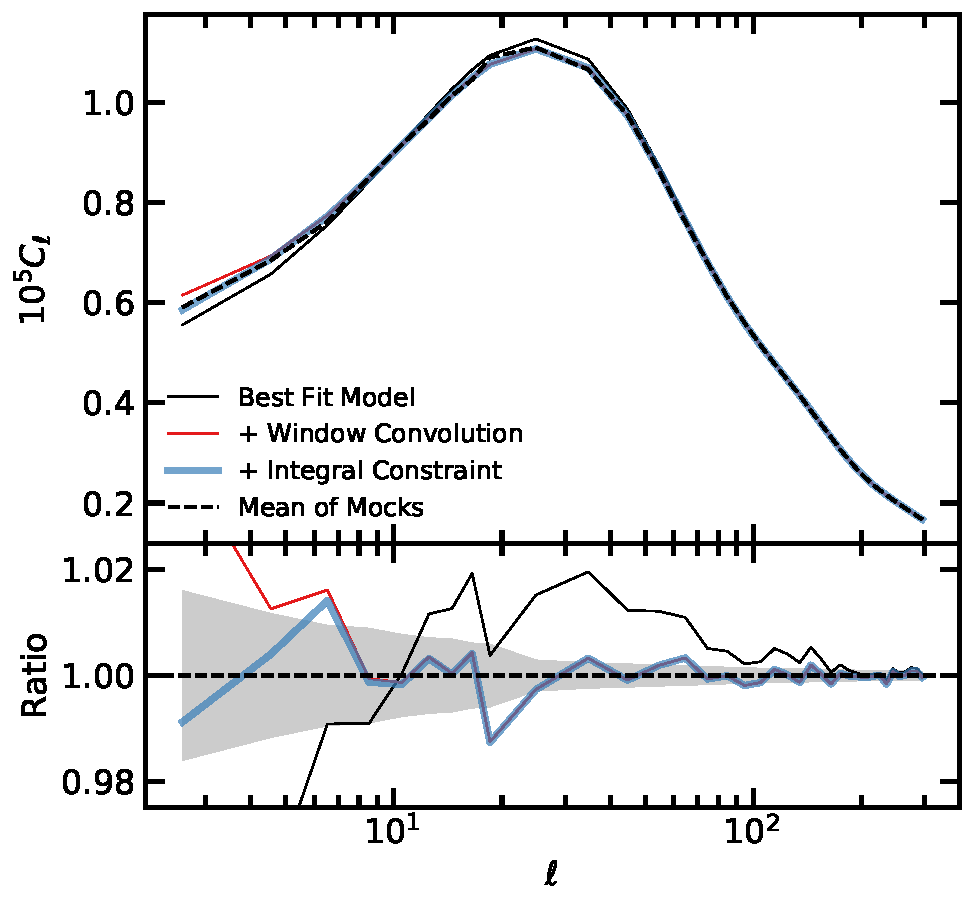
\includegraphics[width=0.5\textwidth]{model_mock.pdf}
\caption{Mean power spectrum of the lognormal density fields with $\fnl=0$ and best fit theoretical prediction after accounting for the survey geometry and integral constraint effects. Dark and light shades represent $1\sigma$ error on the mean and one realization, respectively. Bottom panel shows the residual power spectrum relative to the mean power spectrum of the mocks. No imaging systematic effects are added to these mocks.}\label{fig:model_mock}
\end{figure}

\subsubsection{Survey geometry and integral constraint}
The ensemble average for the partial sky power spectrum is related to that of the full sky power spectrum via the mode-mode coupling matrix $M_{\ell \ell^{\prime}}$ ,
\begin{equation}
    <\hat{C}_{\ell}> = \sum_{\ell^{\prime}} M_{\ell \ell^{\prime}}<C_{\ell^{\prime}}>.
\end{equation}
In general, the mode-mode coupling matrix is singular for a large sky cut, but a common approach is to use a discrete set of $\ell$ bins and assume the angular power spectrum is constant in each bin. This is not a bad assumption, but it might not be ideal for large scale modes and small bin widths. Therefore, we following a similar approach to \cite{chon2004fast}, and convolve the theoretical power spectrum $C_{\ell}$ with the survey mask window power to obtain the theoretical pseudo-power spectrum, rather than trying to de-convolve the observed power spectrum. The convolution in the spherical harmonics space becomes a multiplication in the correlation function space. To this end, we first estimate the paircount of the survey mask. The window paircount is normalized such that it is equal to one at the zero degree separation. Next, we multiply the model correlation function by the survey mask paircount. Then, the window-convolved power spectrum is obtained from,
\begin{align}
    \hat{C}^{\rm model}_{\ell} &= 2\pi \int \hat{\omega}^{\rm model}\hat{\omega}^{\rm mask}~P_{\ell}(\cos \theta) d\theta.
\end{align}

Finally, we account for the effect of integral constraint by subtracting the power spectrum of the survey mask,
\begin{equation}
     \hat{C}^{\rm model, IC}_{\ell} = \hat{C}^{\rm model}_{\ell} - \hat{C}^{\rm model}_{\ell=0} (\frac{\hat{C}^{\rm window}_{\ell}}{\hat{C}^{\rm window}_{\ell=0}}).
\end{equation}

We validate the pipeline for modeling the angular power spectrum against the lognormal simulations. Fig. \ref{fig:model_mock} shows the log-transformed mean of 1000 spectra from the simulations (dashed) and the best fit theory prediction before and after accounting for survey geometry and integral constraint. light and dark shades represent the 68\% error on the mean and one single realization, respectively. DESI footprint mask is applied to the mocks, and even though DESI covers around $40\%$ of the sky, but the window effect is affecting modes down to $\ell=200$. On the other hand, integral constraint only alters the power in the first two bins.

\subsection{Parameter estimation}
The signature of local PNG in the two-point function is unique and cannot be reproduced with other standard cosmological parameters. For parameter inference, we use standard Monte-Carlo Markov Chain sampling while allowing three parameters to vary; $\fnl$, shotnoise, and bias. We assume a constant clustering amplitude for our sample of LRGs, $b(z) = b/D(z)$, and fit for b. Throughout this manuscript, we use a discrete set of bandpower bins with $\Delta\ell=2$ between $\ell=2$ and $20$ and $\Delta \ell=10$ from $\ell=20$ to $300$, while weighting each mode by $2\ell+1$. We also find that the distribution of power spectrum at the lowest bin, $2\leq \ell < 12$,  is not Gaussian and its standard deviation varies significantly from mocks with $\fnl=0$ to those with $76.9$ (see, Fig. \ref{fig:histcell}). Therefore, we attempt to fit $\log C_{\ell}$ to make our constraints less sensitive to the choice of covariance matrix. The parameter $\fnl$ is constrained by maximizing a posterior defined as,
\begin{equation}
-2\ln\mathcal{L} = (\log C(\Theta)-\log \hat{C})^{\dagger} \mathbb{C}^{-1} (\log C(\Theta)-\log \hat{C}) + \chi^{2}_{\rm priors},
\end{equation}
where $\Theta$ represents the parameters, $\fnl$, bias coefficient, and shotnoise, all of which are associated with a flat prior, $\chi^{2}_{\rm priors}$; $C(\Theta)$ is the (binned) theoretical power spectrum including the effects for survey geometry and integral constraint; $\hat{C}$ is the (binned) measured power spectrum; and $\mathbb{C}$ is the covariance matrix constructed from simulations. 

\begin{figure}
\centering
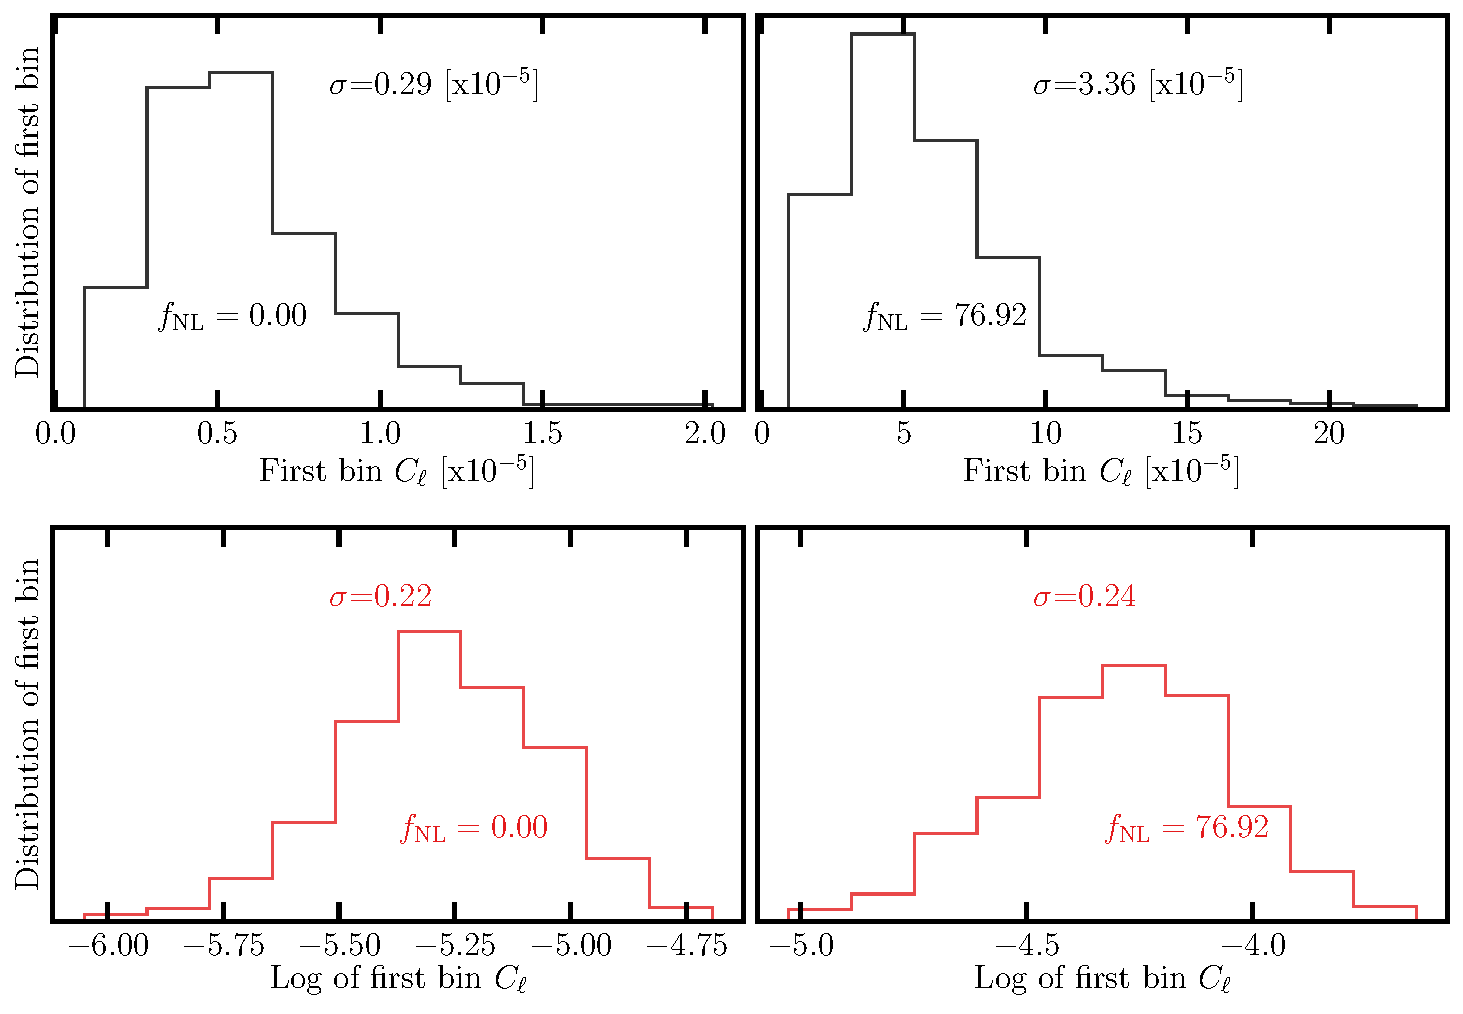
\includegraphics[width=0.5\textwidth]{hist_cl.pdf}
\caption{Distribution of the first bin power spectrum and its log transformation from the mocks with $\fnl=0$ (left) and $76.92$ (right). Differences in the standard deviations become less significant, and power spectrum measurements follow a more symmetric distribution after the log transformation.}\label{fig:histcell}
\end{figure}


\subsection{Remaining systematic errors}
\label{ssec:characterization}


We use the diagnostic tests first applied to SDSS data in \cite{rezaie2021primordial} based on cross power spectrum between galaxy density field and imaging maps and mean density contrast as a function of imaging properties to quantify the significance of imaging systematic effects. 

\begin{figure*}
\centering
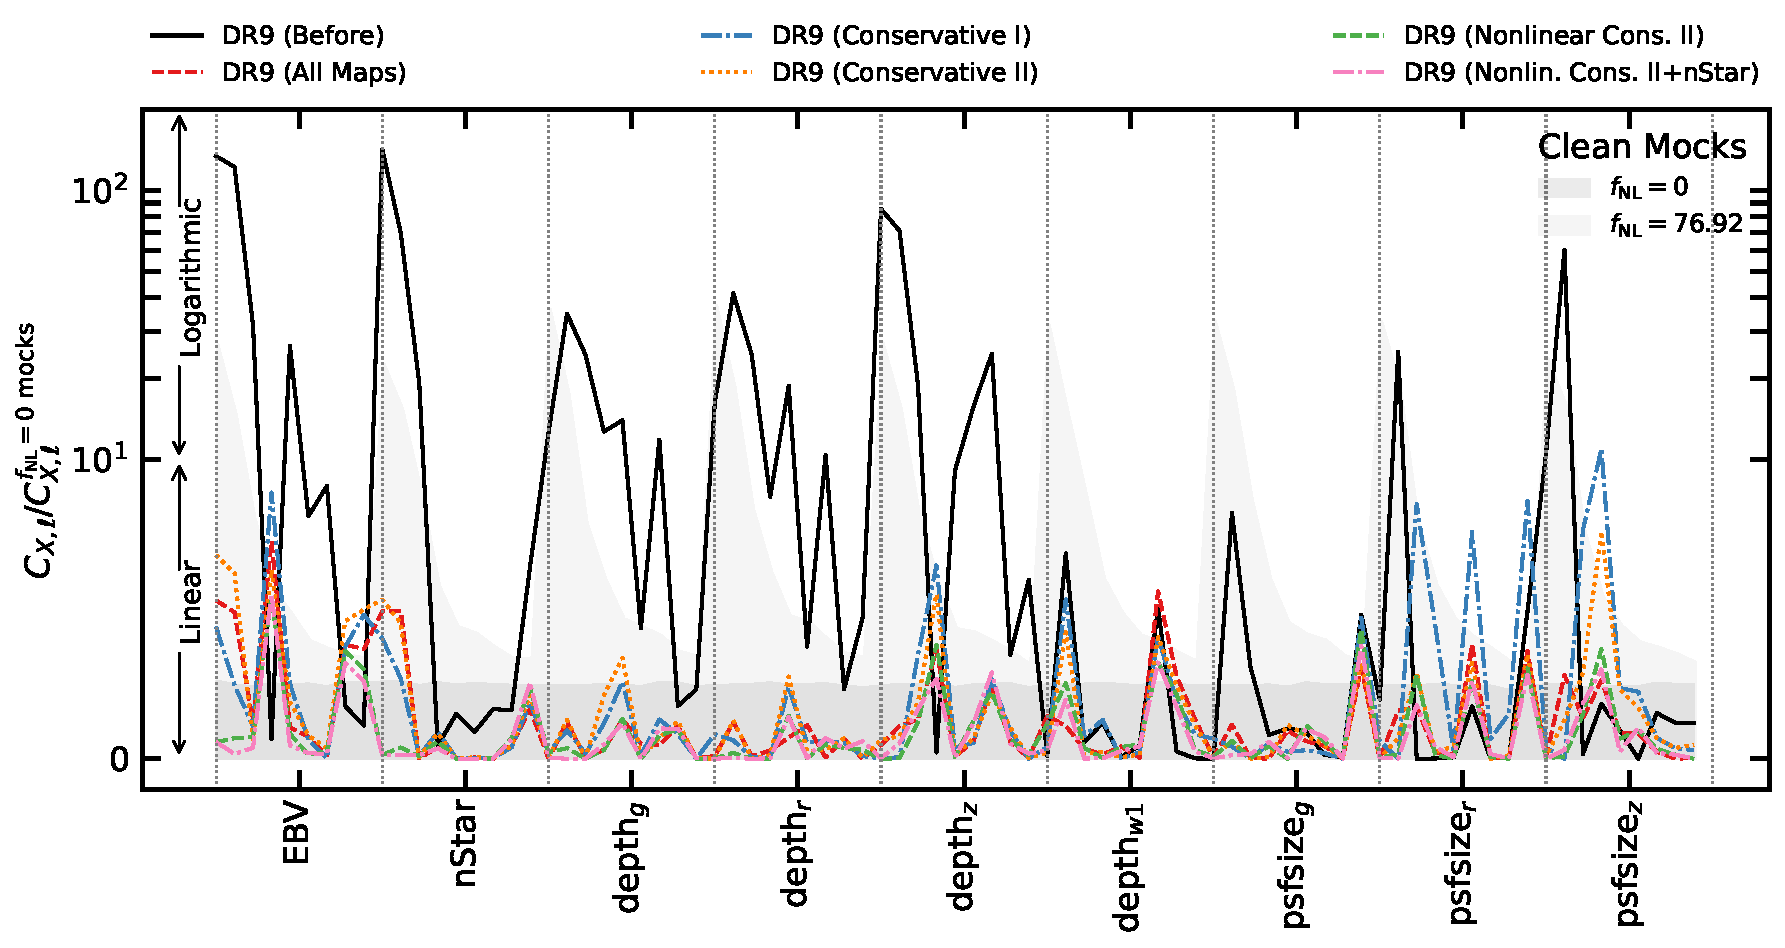
\includegraphics[width=0.76\textwidth]{clx_mocks.pdf}
\caption{Cross power spectra between the DR9 LRG sample and imaging maps. Dark and light shades represent the $97.5$ percentile of 1000 lognormal mocks without and with PNG, respectively.}\label{fig:clxmock}
\end{figure*}

\begin{figure*}
\centering
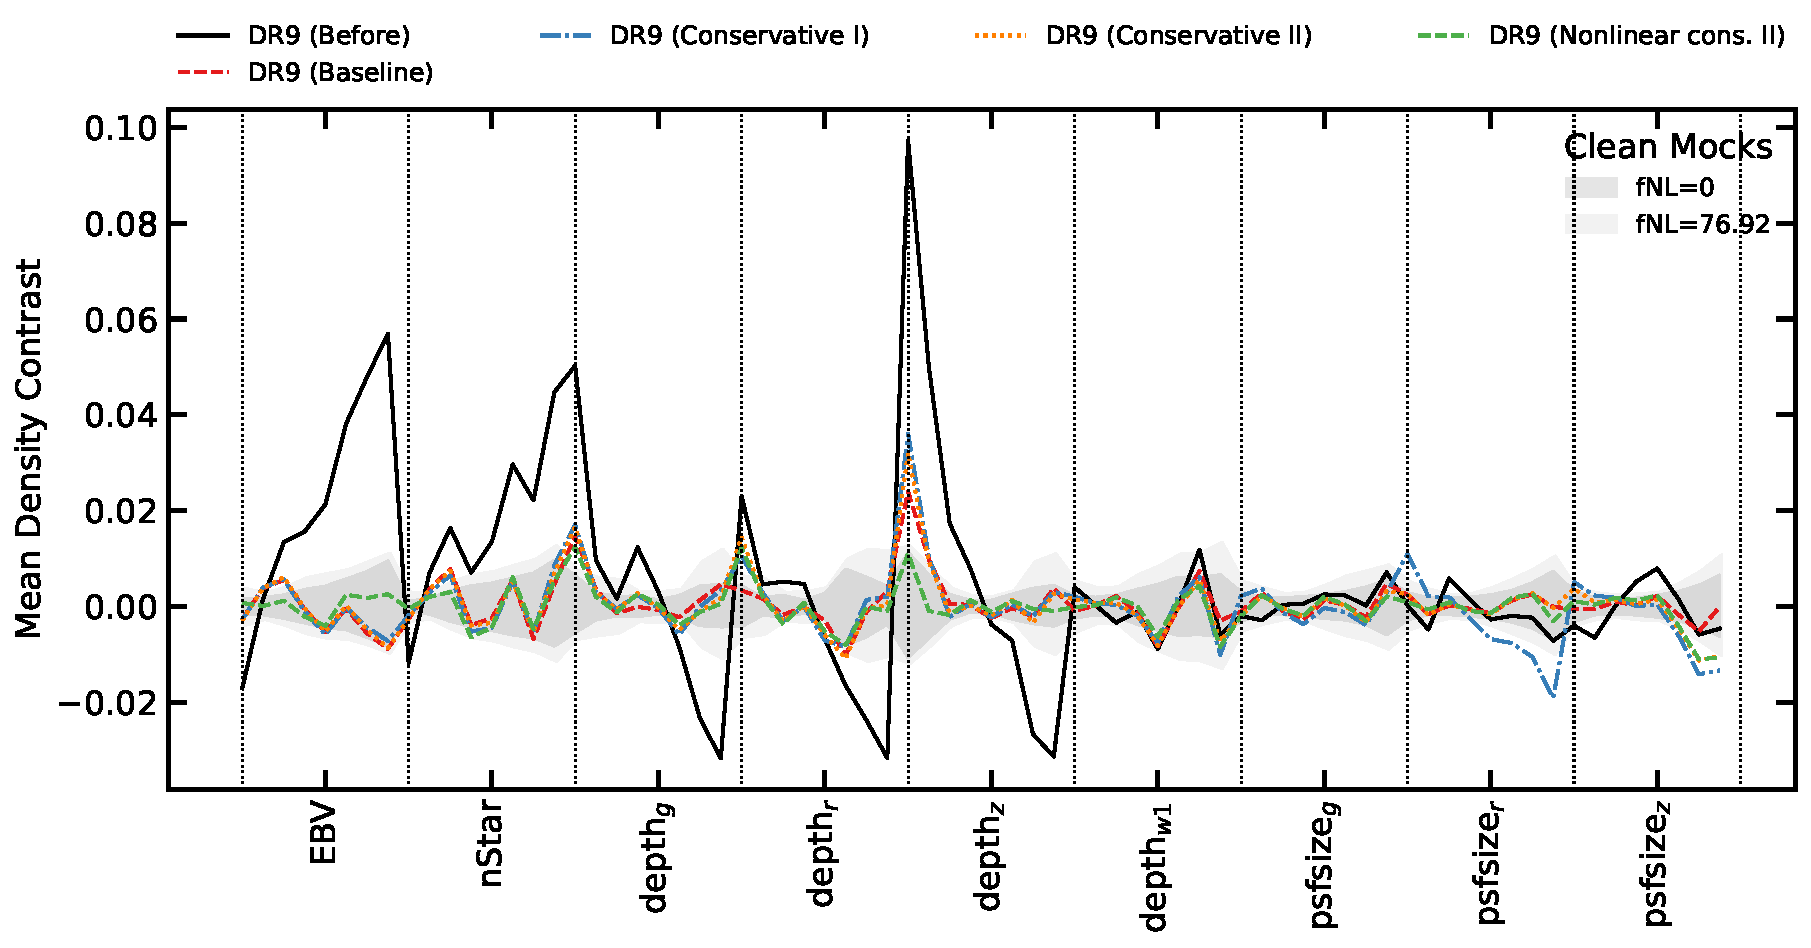
\includegraphics[width=0.76\textwidth]{nbar_mocks.pdf}
\caption{Mean density contrast of the DR9 LRG sample as a function of imaging maps. Dark and light shades represent the $1\sigma$ dispersion of 1000 lognormal mocks without and with PNG, respectively.}\label{fig:nbarmock}
\end{figure*}


\begin{figure}
\raggedleft
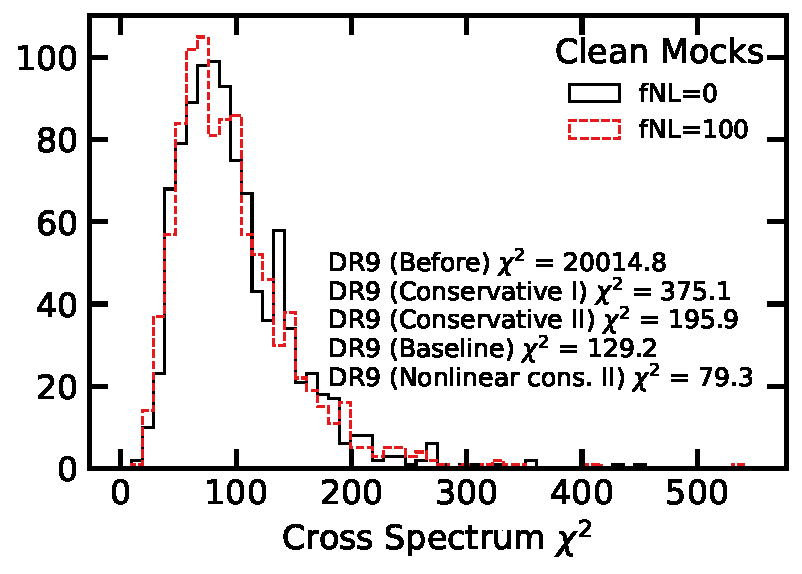
\includegraphics[width=0.45\textwidth]{chi2test.pdf}
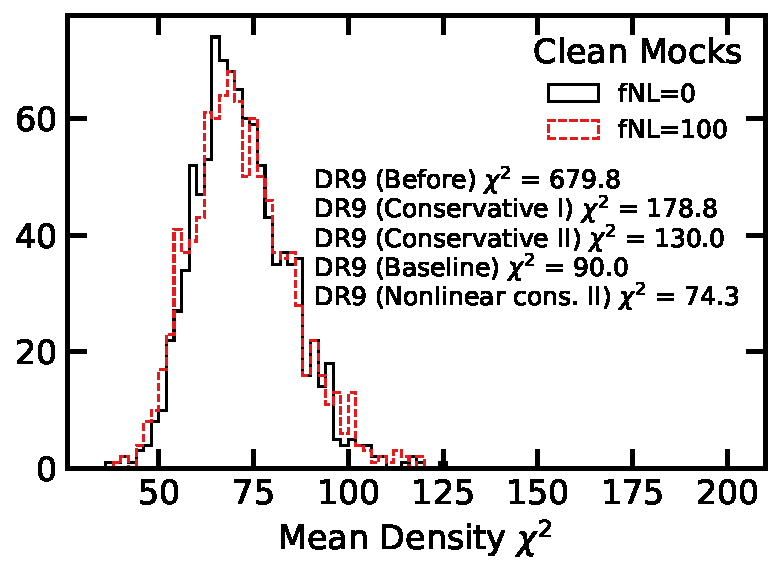
\includegraphics[width=0.44\textwidth]{chi2test2.pdf}
\caption{Remaining systematic error $\chi^{2}$ from the galaxy-imaging cross power spectrum (top) and the mean galaxy density contrast (bottom). The values observed in the DR9 sample before and after linear and nonlinear treatments are quoted, and the histograms are constructed from 1000 realizations of clean lognormal mocks with $\fnl=0$ and $76.92$.}\label{fig:chi2test}
\end{figure}

\begin{figure}
\centering
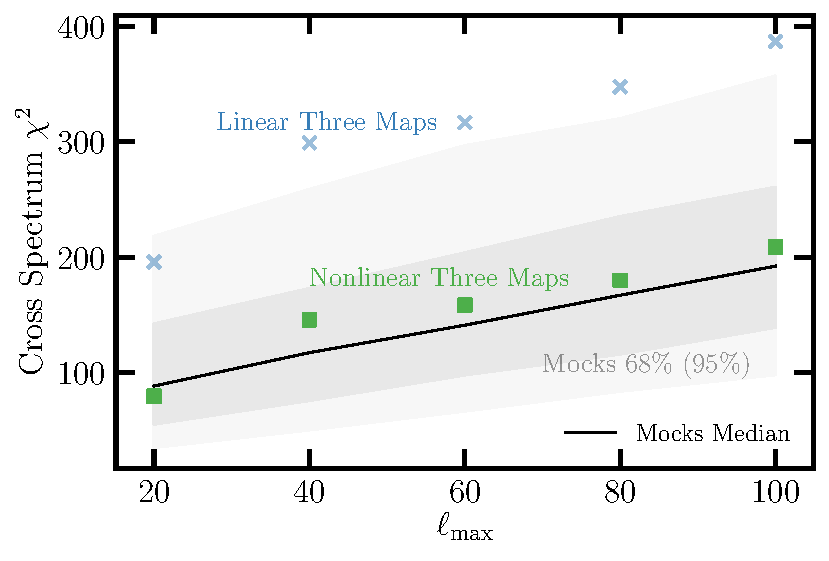
\includegraphics[width=0.5\textwidth]{chi2lmax.pdf}
\caption{Cross power spectrum $\chi^{2}$ as a function of the highest mode $\ell_{\rm max}$ for the DR9 LRG sample using the linear and nonlinear imaging weights with the conservative II maps. The lowest mode is fixed at $\ell_{\rm min}=2$. Solid curve and dark (light) shade represent the median estimate and $68\%$ ($95\%$) confidence constructed from the $\fnl=0$ mocks.}\label{fig:chi2cellextend}
\end{figure}


\subsubsection{Cross power spectrum}
Taking $C^{g,x}_{\ell}$ as the cross power spectrum between galaxy density contrast field and imaging map, one can normalize this quantity by auto power spectrum of imaging map itself:
\begin{equation}
\hat{C}_{x, \ell} = \frac{(\hat{C}^{g,x}_{\ell})^{2}}{\hat{C}^{x,x}_{\ell}},
\end{equation}
and then construct a vector from cross spectra against all other imaging maps:
\begin{equation}
\hat{C}_{X, \ell} = [\hat{C}_{x_{1}, \ell}, \hat{C}_{x_{2}, \ell}, \hat{C}_{x_{3}, \ell}, ..., \hat{C}_{x_{9}, \ell}].
\end{equation}
Finally, cross power spectrum $\chi^{2}$ can be defined as,
\begin{equation}
\chi^{2} = C^{T}_{X, \ell} \mathbb{C}_{X}^{-1} C_{X, \ell},
\end{equation}
where covariance matrix $\mathbb{C}_{X} = < C_{X, \ell} C_{X, \ell'} >$ is constructed from mocks without systematic effects. This statistics is measured for every mock realization with the leave-one-out technique to construct a histogram, which is then compared to the $\chi^{2}$ value observed from the DR9.  Fig. \ref{fig:clxmock} (top) shows the measured $C_{X}$ the DR9 sample before and after applying various imaging weights, relative to that of the mocks with $\fnl=0$. The dispersions of mocks with and without PNG are shown with the shade regions for comparison. We bin the $C_{X}$ measurements from $\ell=2$ to $20$ with $\Delta\ell=2$. The mean and standard deviation of $\hat{C}_{X, \ell}$ for 1000 mocks with and without $\fnl$ are shown in Fig. \ref{fig:clxmock}.  Extinction and stellar density have the highest cross power spectrum, and then depth in the z band. After applying the first version of weights with linear conservative I which includes extinction and depth-z, the cross power increases against psftsize in the r band. This indicates that only two maps are not sufficient to null out all of the cross correlations. With linear model there is residual power against extinction, depth-z, and psfsize-z; therefore, we apply weights based on a nonlinear model to account for more complex systematic effects. 

Fig. \ref{fig:chi2test} (top) shows the histogram of cross spectrum $\chi^{2}$ from mocks with and without $\fnl$. Comparing with the data, the residual is 20014.8 before correction, and after applying the first set of weights, it reduces to 375.1 with p-value \mr{XXX}. Adding psfsize-z, the linear model reduces the error dow to 195.9 (\mr{p-value = XXX}). Although using all maps gives the lowest error i.e., 129.2, but it could potentially lead to over-fitting true clustering given how correlated the imaging maps are (see, Fig. \ref{fig:pcc}). On the other hand, the nonlinear method with three maps yields a $\chi^{2}$ value of 79.3 and p-value of XXX, and adding the stellar density map reduces the error to 70.9 (p-value=XXX). This test clearly shows that a nonlinear approach is desired to get a null test. We further test the stability of our results by extending the highest mode from $\ell=20$ to $100$, or fluctuations over scales as small as $1.8$ degrees (see, Fig. \ref{fig:chi2cellextend}). The solid line shows how the median of 1000 mocks changes as the highest $\ell$ increases from $20$ to $100$. The red circles show the chi2 for the linear approach with three maps and the blue crosses show the chi2 for the nonlinear approach with three maps.

\subsubsection{Mean density contrast}
In the absence of systematic error, the integral of mean density contrast over the footprint should be zero As an alternative test, we calculate the histogram of the density contrast field relative to each imaging map.
\begin{equation}
\delta_{x} = ({\hat{\overline{\rho}}})^{-1} \frac{\sum_{i} \rho_{i} f_{{\rm pix}, i}}{\sum_{i} f_{{\rm pix}, i}},
\end{equation}
where the summations are over pixels in each bin of imaging map $x$. Similarly, we construct the mean density contract vector against all imaging maps,
\begin{equation}
\delta_{X} = [\delta_{x_{1}}, \delta_{x_{2}}, \delta_{x_{3}}, ..., \delta_{x_{9}}],
\end{equation}
and the total residual error as,
\begin{equation}
\chi^{2} = \delta_{X}^{T} \mathbb{C_{\delta}}^{-1} \delta_{X},
\end{equation}
where the covariance matrix $\mathbb{C}_{\delta} = < \delta_{X} \delta_{X}>$ is constructed from mocks without systematic effects. Fig. \ref{fig:clxmock} (bottom) shows the mean density contrast for the DR9 LRG sample. The shades represent the $1\sigma$ level fluctuations observed in 1000 clean mocks with $\fnl=0$ and $76.92$. Before treatment (solid) shows strong correlation around $10\%$ against depth in the z band which is consistent with the cross power spectrum. Beside that, there are strong positive trends against extinction and stellar density at about $5-6\%$. The linear model is able to mitigate most of the systematic effects with only the extinction and depth-z maps as input, however a new trend appears against psfsize-r which is indicative of psfsize dependence in the sample. This finding is in agreement with the cross power spectrum. Even after applying the linear weights there is some residual against depth-z at around $2\%$, which indicates the systematic effects might be more complex than what can be removed using a linear model. Nonlinear model with three maps (or four maps including the stellar density) is capable of reducing the fluctuations below $2\%$. 


Fig. \ref{fig:chi2test} (bottom) shows the mean density $\chi^{2}$ observed in the mocks vs DR9 sample before and after applying imaging weights. Linear weights with two maps reduce the chi-2 value from 679.8 (before) to 178.8. The p-value is indicative of remaining systematic effects. Adding psfsize-r does not help much with the p-value even though it reduces the chi-2 to 130. Using all maps with the linear model gives a more reasonable value however it leaves the analysis susceptible to over-fitting true clustering signal. With nonlinear approach two maps as input, the chi-2 is reasonable 74.3 with p-value XXX, and adding the stellar map does not change the p-value much, indicating the trend against stellar density can be explained with the extinction to a great extend. 